% Dokumentation von Julian Sehbaoui%

%Set the documentclass to article with a4 paper and 10pt font%
\documentclass[a4paper, 10pt]{scrartcl}

%importing german packages%
\usepackage[ngerman]{babel}
\usepackage[utf8]{inputenx}
\usepackage[T1]{fontenc}

%importing the other packages%
\usepackage{amsmath}
\usepackage{xcolor}
\usepackage{hyperref}
\usepackage{listings}
\usepackage{enumerate}
\usepackage{graphicx}
\usepackage{fancyhdr}
\usepackage{sidecap}
\usepackage{placeins}
\usepackage{wrapfig}
\usepackage[export]{adjustbox}
\usepackage{tikz-uml}

\sidecaptionvpos{figure}{t}

%setting the listing package settings for later code blocks%
\lstset{frame=tb,
  language=Python,
  aboveskip=3mm,
  belowskip=3mm,
  showstringspaces=false,
  columns=flexible,
  basicstyle={\small\ttfamily},
  numbers=none,
  numberstyle=\tiny\color{gray},
  keywordstyle=\color{blue},
  commentstyle=\color{green},
  stringstyle=\color{purple},
  breaklines=true,
  breakatwhitespace=true,
  tabsize=3
}

%creating the header and footer%
\pagestyle{fancy}
\fancyhf{}
\lhead{Julian Sehbaoui}
\chead{\glqq Schach.py\grqq{}}
\rhead{Luisengymnasium Bergedorf}
\rfoot{Seite \thepage}
\renewcommand{\headrulewidth}{2pt}

%setting document attributes for the titlepage%
\title{Informatik Dokumentation "Schach.py"}
\author{Julian Sehbaoui}
\date{\today}

%begin the document
\begin{document}

%create the titlepage%
\begin{titlepage}
        \maketitle
        \centering
        \url{https://github.com/JSehbaoui/Chess_Python}\\
         \vspace{5pt} 
        
\includegraphics[scale=0.35]{assets/luisengymnasium.png}\\
         \vspace{5pt} 
        
        Made with \LaTeX{}
\end{titlepage}

%creating a single page just for the table of contents%
\pagebreak
\tableofcontents
\pagebreak

%THE DOCUMENTATION:%
\section{Vorwort}
Dieses Projekt findet im Rahmen des Informatikunterrichts des Luisengymnasiums 	Bergedorf statt und wird als zusätzliche Lernleistung entsprechend gewertet.
Ich bin Julian Y. Sehbaoui und habe ein Schachprogramm „from scratch“ in python3 geschrieben.

\section{Das Ziel}
Mein Ziel war es ein vollfunktionalles Schachspiel ausschließlich in Python
zu erschaffen, welches alle klassischen Regeln des Schachs beachtet. 
Hierbei wollte ich auf jegliche äußerliche Hilfe, wie zum Beispiel API's oder schon
existierende Algorhytmen verzichten, mit Ausnahme eines Schachcomputers. 
Außerdem soll man zwischen PvP (Player versus Player) und PvE (Player versus)

\section{Ideenfindung}
Ich persönlich habe mich schon seit dem ich klein bin für Schach interessiert.
Es ist ein recht simples Spiel, welches aber durch seine Zahlreichen Zugmöglichkeiten zu einem sehr tiefgründigen Spiel werden kann.
Als ich mich nach einem neuen Projekt umgesehen habe, kam mir direkt Schach in den Sinn, weil es an strikte Regeln gebunden ist, nicht viele Ausnahmen existieren
und ich es wie schon erwähnt sehr gerne spiele.

%\section{Die Regeln im Schach}
%Im Folgenden finden Sie alle offiziellen Regeln des standartmäßigen Schachspiels
%
%\subsection{Das Spielprinzip}
%Ein Schachspiel wird zwischen zwei Gegnern ausgetragen, die ihre Spielfiguren auf einem quadratischen Spielbrett ziehen. 
%Das Ziel des Spiels für beide Spieler ist es den gegnerischen König „Schachmatt“ zu setzten. Dieser Zustand ist erreicht, wenn der gegnerische Spieler keine Möglichkeit hat, den König mit dem nächsten Zug aus dem „Schach“ (angegriffener Zustand des Königs) zu bewegen. 
%Falls es für keinen der Beiden Spieler möglich ist den Gegner Schachmatt zu setzten, wird das Spiel mit einem Remis (=Unentschieden/Gleichstand) beendet.
%
%\subsection{Anfangsstellung der Figuren}
%Das Schachbrett besteht aus einem 8x8 Gitter mit 64 gleichgroßen Quadraten, welche abwechselnd hell und dunkel sind (meist weiß und schwarz).
%Die Spieler positionieren sich gegenüber voneinander, sodass bei beiden Spielern ein weißes Feld in der unteren rechten Ecke vorhanden ist.
%Zu Beginn des Spiels hat jeder Spieler 16 Figuren; Ein Spieler die die Hellen (weiß) und einer die Dunklen (schwarz).
%Beide Spieler starten mit 8 Bauern, 2 Türmen, 2 Springern, 2 Läufern, einer Dame und einem König.
%Die Figuren sind wie folgt anzuordnen:
%
%\begin{figure}
%        \centering
%        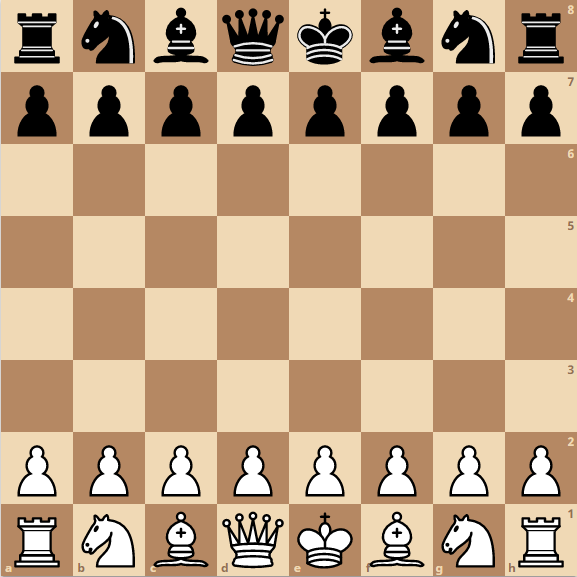
\includegraphics[scale=0.5]{assets/chess-opening.png}
%        \caption{Anfangsaufstellung der Schachfiguren im Standardschach}
%\end{figure}
%
%
%Die senkrechten Spalten sind die „Linien“, die waagerechten Zeilen sind die „Reihen“ und die gradlinige Folge der Felder, die sich an den Ecken Berühren sind die „Diagonalen“.
%
%\subsection{Gangart der Figuren}
%Allgemeingültige Regeln sind folgende:
%\begin{itemize}
%        \item Eine Figur darf nicht auf das Feld einer verbündeten Figur ziehen
%        \item Es ist nicht möglich eine Figur durch ein Feld hindurch zu ziehen, welches von einer anderen Figur besetzt ist (Ausnahme siehe 3.3.4.)
%        \item Wenn eine Figur auf ein Feld zieht, welches von einer gegnerischen Figur besetzt ist, dann wird die Gegnerfigur geschlagen (=entfernt)
%        \item Keine Figur darf einen Zug machen, welcher den eigenen König einem Schachgebot aussetzt oder ihn in einem Schachgebot stehen lässt.
%    
%\end{itemize}
%
%\subsubsection*{Läufer}
%\begin{SCfigure}[4][h]
%        \caption{\protect\rule{0ex}{4ex}
%        Der Läufer darf auf ein beliebiges 
%        Feld entlang der Diagonale ziehen, auf der er steht.
%        }
%        
\includegraphics[width=0.15\textwidth]{assets/bishop_split.png}
%\end{SCfigure}
%
%\pagebreak
%
%\FloatBarrier
%\subsubsection*{Turm}
%\begin{SCfigure}[4][h]
%        \caption{\protect\rule{0ex}{4ex}
%        Der Turm darf auf ein beliebiges Feld 
%        entlang der Linie oder der Reihe ziehen, auf der er steht.
%        }
%        
\includegraphics[width=0.15\textwidth]{assets/rook_split.png}
%\end{SCfigure}
%
%\FloatBarrier
%
%\subsubsection*{Dame}
%\begin{SCfigure}[4][h]
%        \caption{\protect\rule{0ex}{4ex}
%        Die Dame darf auf ein beliebiges Feld 
%        entlang der Linie, Reihe oder Diagonalen ziehen, auf der die steht.
%        }
%        
\includegraphics[width=0.15\textwidth]{assets/queen_split.png}
%\end{SCfigure}
%
%\subsubsection*{Springer}
%\begin{SCfigure}[4][h]
%        \caption{\protect\rule{0ex}{4ex}
%        Der Springer darf auf eines der Felder ziehen, 
%        die seinem Standfeld am nächsten, aber nicht auf gleicher Linie, 
%        Reihe oder Diagonalen mit diesem liegen.
%        }
%        
\includegraphics[width=0.15\textwidth]{assets/knight_split.png}
%\end{SCfigure}
%
%\subsubsection*{Bauer}
%
%\begin{wrapfigure}{l}{0.28\textwidth}
%        
\includegraphics[width=0.15\textwidth, right]{assets/pawn_split.png}
%\end{wrapfigure}
%Der Bauer darf
%\begin{itemize}
%        \item vorwärts auf das unbesetzte Feld direkt vor ihm auf derselben Linie ziehen
%        \item in seinem ersten Zug entweder wie unter (a) beschrieben ziehen oder um zwei Felder entlang derselben Linie vorrücken, vorausgesetzt, dass beide Felder frei sind, oder
%        \item auf ein von einer gegnerischen Figur besetztes Feld diagonal vor ihm auf einer benachbarten Linie ziehen, indem er jene Figur schlägt.
%        \item sobald er diejenige Reihe erreicht hat, die am weitesten von seinem Ursprungsfeld entfernt ist, muss er sich als Teil desselben Zuges gegen eine Dame, einen Turm, einen Läufer oder einen Springer derselben Farbe austauschen. Die Auswahl des Spielers ist nicht auf bereits geschlagene Figuren beschränkt. Dieser Austausch eines Bauern für eine andere Figur wird «Umwandlung» genannt, und die Wirkung der neuen Figur tritt sofort ein.
%\end{itemize}
%
%
%\subsubsection*{König}
%
%\begin{wrapfigure}{l}{0.28\textwidth}
%        
\includegraphics[width=0.15\textwidth, right]{assets/king_split.png}
%\end{wrapfigure}
%Es gibt zwei verschiedene Arten den König zu ziehen:
%\begin{enumerate}
%        \item Er zieht auf ein beliebiges angrenzendes Feld, das nicht von einer oder mehreren gegnerischen Figuren angegriffen wird. Von den gegnerischen Figuren gilt, dass sie ein Feld auch dann angreifen, wenn sie selbst nicht ziehen können. Oder
%        \item er «rochiert». Die «Rochade» ist ein Zug des Königs und eines gleichfarbigen Turmes auf der gleichen Reihe. Sie gilt als ein einziger Zug und wird folgendermaßen ausgeführt: Der König wird von seinem Ursprungsfeld um zwei Felder in Richtung des Turmes hin versetzt, dann wird dieser Turm auf das Feld gesetzt, das der König soeben überquert hat.
%        \begin{enumerate}
%                \item Die Rochade ist regelwidrig:
%                \begin{enumerate}
%                        \item wenn der König bereits gezogen hat, oder
%                        \item mit einem Turm, der bereits gezogen hat.
%                \end{enumerate}
%                \item Die Rochade ist vorübergehend verhindert,
%                \begin{enumerate}
%                        \item wenn das Standfeld des Königs oder das Feld, das er überqueren muss, oder sein Zielfeld von einer oder mehreren gegnerischen Figuren angegriffen wird,
%                        \item wenn sich zwischen dem König und dem Turm, mit dem rochiert werden soll, irgendeine Figur befindet.
%                \end{enumerate}
%        \end{enumerate}
%\end{enumerate}
%Ein König «steht im Schach», wenn er von einer oder mehreren gegnerischen Figuren angegriffen wird, auch wenn diese selbst nicht ziehen können.
%
%\subsection{Ende der Partie}
%Eine Partie endet entweder durch ein „Schachmatt“ oder durch ein „Remis“ (siehe 3.1.).
%Eine Partie kann auch durch eine Übereinstimmung beider Spieler mit einem Remis entschieden werden. 
%Ein Ende Partie ist auch durch eine dreifach wiederholte identische Zugfolge mit einem Remis zu beenden. 
%Falls 50 Züge ohne einen Bauernzug oder das schlagen einer Figur vergehen, ist dies ebenfalls ein Unentschieden.

\section{Benutze Pakete}
Im Folgenden finden sie die verwendeten Pakete, sowie die Vorteile, welche mich zu der Entscheidung geführt haben.

\subsection{pygame}
„pygame“ ist eine Ansammlung von Python-Modulen welche auf das programmieren von Videospielen ausgelegt sind. Es ist auf sämtlichen OS verfügbar und hat schon mehrere Millionen Benutzer.

\subsubsection{Warum pygame?}
„pygame“ ist aufgrund der großen Community sehr gut dokumentiert.
Außerdem bietet es eine wundervolle SDL (Simple Direct Media) Bibliothek.
Ein weiterer Grund für die Verwendung von pygame war, dass ich schon ein
wenig Erfahrung mit dem Modul sammeln konnte und daher für mich die erste
oberflächliche Benutzung erleichtert wurde.
Eine Alternative für mich war die \href{https://processing.org/}{Processing}.
Processing ist ein \glqq Scetchbook \grqq , welches einem erlaubt
auf einer graphischen Oberfläche zu programmieren. Es ist ein leichtverständliches
Prinzip, da man hier mit der Syntax von entweder Java oder Python funktionell programmieren
kann. Außerdem, da Processing für graphische Arbeiten und kleine Spiele geschaffen wurde,
lässt sich schnell und einfach die Mausposition und weitere Inputs abfragen und
Figuren und Bilder auf der graphischen Oberfläche abbilden.
Des Grund warum ich mich dennoch für pygame entschieden habe war, dass man in pygame
Objektorientiert arbeiten kann. Kurz gesagt verwendet man bei der Objektorientierten Programierung
Grundgerüste (sogenannte Klassen), mitwelchen sich Objekte mit durch die Klasse definierten Attributen
erstellen lassen. Dieses Konzept ist hilfreich bei der Programmierung eines Schachspiels,
da sich alle Figuren an den selben \glqq Bauplan\grqq halten und sich über das Prinzip der Vererbung
sich die Figurtypischen Eigentschaften in dieses Grundgerüst implementieren lassen.

\subsection{Stockfish}
Stockfish ist eine berühmte Schachengine, welche von vielen großen Schachanalysten und Schachwebsites benutzt wird.

\subsubsection{Warum Stockfish?}
Stockfish hat eine gute Python Unterstützung. Außerdem ließ es sich nach ein paar wenigen Komplikationen auch gut benutzen und implementieren.

\section{Installation}
Mein Skript ist kostenlos von der Seite \href{https://github.com/Aetherion-dot/Chess_Python}{\color{blue}{github}} herutergeladen werden.
Offensichtlicher Weise muss man um das Python-Skript auszuführen, \href{https://www.python.org/downloads/}{\color{blue}{python3}} herunter laden. 
Um dieses dann zu starten sind die Pakete „Stockfish“, „pygame“ und "pygame-widgets" über \href{https://pypi.org/project/pip/}{\color{blue}{pip}} herunter zuladen.
Dies ist über die Konsole mit den Befehlen
\begin{lstlisting}[language=bash]
        pip install pygame
\end{lstlisting}
\begin{lstlisting}[language=bash]
        pip install stockfish
\end{lstlisting}
\begin{lstlisting}[language=bash]
        pip install pygame-widgets
\end{lstlisting}
zu erreichen.

\section{Bedienung des Programmes}
%BILDER
\subsection{Wie spiele ich?}
Um das Schachprogramm zu starten muss man die \glqq init.py\grqq Datei in python starten. Anschließend öffnet sich ein Fenster, in welchem man zwischen verschiedenen Spielmodi
wählen kann.

\begin{figure}
        \centering
        %\includegraphics{assets/}
\end{figure}

Die beiden Modi die hier zur Auswahl stehen sind einmal die Standard-Schach-Variante und die Chess 960 Variante, bei der die Figuren in der hinteren Reihe
zufällig angeordnet werden.
Für jeden der beiden Modi lässt sich optional ein zweiter virtueller Spieler hinzufügen, falls man keinen realen Gegner bei sich hat.
Nachdem man sich für einen Modus entschieden hat, lässt sich der Spielername und je nach Option die Computerschwierigkeit oder der Name des zweiten Spielers einstellen.
Nun kann das Spiel durch den Knopf unterhalb der Einstellungen gestartet werden und das tatsächliche Spiel kann beginnen.
Sobald man auf eine Figur klickt, öffnen sich auf dem Feld alle legalen Zugoptionen. Wenn man anschließend auf ein Feld klickt, welches die Figur betreten kann, bewegt
sich die ausgewählte Figur auf das gewünschte Feld.

\subsection{Overlays}

\subsubsection{Spielerinformationstabs}
Im oberen Bereich des Spielfelds befindet sich zum einen eine Uhr, welche die aktuelle Spielzeit anzeigt. Links und rechts danaben befinden sich die Spielerinformationen.

\begin{figure}[h]
        \centering
        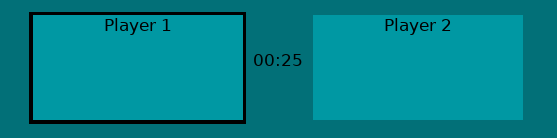
\includegraphics[scale=0.7]{assets/infotabs.PNG}
        \caption{Informations-Tabs und Spielzeit}
\end{figure}
In diesen werden die geschlagenen Figuren sowie der Spielername angezeigt. Außerdem wird das Spielerinformationsfeld von dem Spieler hervorgehoben, welcher daram ist, den
nächsten Zug zu machen.

\subsubsection{Spielhistorie}

In dem rechten Teil des Fensters befindet sich die Spielhistorie. Diese zeigt die bereits gezogenen Spielzüge an. 

\subsubsection{Buttons}
Oben im rechten Eck finden sich insgesammt drei Buttons mit folgenden Funktionen:
\begin{wrapfigure}{r}{0.5\textwidth}
        \centering
        
\includegraphics{assets/Buttons.PNG}
        \caption{Bedienungs-Knöpfe}
\end{wrapfigure}

\begin{itemize}
        \item \glqq Quit\grqq-Button
        \begin{itemize}
                \item Der Quit-Button beendet sofort das Spiel und schließt das Fenster.
        \end{itemize}
        \item \glqq Resign\grqq-Button
        \begin{itemize}
                \item Beendet das Spiel mit einem Sieg für den anderen Spieler
        \end{itemize}
        \item \glqq Takeback\grqq-Button
        \begin{itemize}
                \item Macht den letzten Zug rückgängig
                \item Ist nur zu benutzen, wenn keine Figur im 
                letzten zug geschlagen wurde, um große Patzer zu bestrafen.
        \end{itemize}
\end{itemize}



\section{Code}
In dem folgenden Kapitel werde ich das Konzept meines Codes erläutern und die Entwicklung darstellen. 

\pagebreak
\subsection{Klassenbeziehungen}

\begin{figure}[!h]
\begin{center}
\begin{tikzpicture}
%\begin{umlpackage}{Chess}
\begin{umlpackage}{Figuren}
\umlclass{Pieces}{
	master : pygame.Surface \\ 
	name : String \\
	tile x : int \\
	tile y : int \\
	color : Tuple \\
	image : pygame.image \\
	value : int 
}{
        draw() : void \\
        animate() : void \\
        move() : void \\
        foresight() : bool \\
}
\umlclass[x=-3,y=-5]{BlackPawn}{}
{
        getPossibleMoves() : array \\
        promotion() : void \\
        attacked\_tiles : array
}
\umlclass[x=3,y=-5]{WhitePawn}{}
{
        getPossibleMoves() : array \\
        promotion() : void \\
        attacked\_tiles : array
}
\umlclass[x=-3,y=-7.5]{Knight}{}
{
        getPossibleMoves() : array \\
        attacked\_tiles : array
}
\umlclass[x=3,y=-7.5]{Bishop}{}
{
        getPossibleMoves() : array \\
        attacked\_tiles : array
}
\umlclass[x=-3,y=-10]{Rook}{}
{
        getPossibleMoves() : array \\
        attacked\_tiles : array
}
\umlclass[x=3,y=-10]{Queen}{}
{
        getPossibleMoves() : array \\
        attacked\_tiles : array
}
\umlclass[x=0,y=-12.5]{King}{}
{
        getPossibleMoves() : array \\
        attacked\_tiles : array
}
\umlinherit[geometry = |-]{Pieces}{WhitePawn}
\umlinherit[geometry = |-]{Pieces}{BlackPawn}
\umlinherit[geometry = |-]{Pieces}{Knight}
\umlinherit[geometry = |-]{Pieces}{Bishop}
\umlinherit[geometry = |-]{Pieces}{Rook}
\umlinherit[geometry = |-]{Pieces}{Queen}
\umlinherit{Pieces}{King}

\end{umlpackage}

%\begin[x=5,y=0]{umlpackage}{Tools}
%\umlclass{Button}
%{command : funktion}
%{draw() : void \\
%processEvent(event : pygame.Event) : void}
%
%\umlclass[x=0, y=-3]{Entry\_Box}
%{}
%{draw() : void \\
%export() : any}
%        
%\end{umlpackage}

%\umlclass[x=5, y=-10]{Board}
%{tile\_size : int}
%{drawBoard() : void}

%\end{umlpackage}
\end{tikzpicture}
%\caption{UML-Diagram der Figurenklassen}
\end{center}
\end{figure}

Oben zu sehen ist ein UML-Diagramm um die Beziehungen von den verschiedenen
Klassen zu visualisieren. Zu erkennen ist eine Parentclass \glqq{}Pieces\grqq ,
welche alle Methoden enthällt, die für eine beliebige Schachfigur von nöten sind.
Von dieser Klasse erben insgesammt sieben andere Klassen. Jede Klasse hat ihre eigene
Methode, um die möglichen Züge zu berechnen. Getrennt sind hierbei die Bauern, in
BlackPawn und WhitePawn. Das war nötig, da sich die Bauern der verschiedenen Teams als
einzige Figur nicht exakt so wegbewegt, wie die des gegnerischen Teams. So bewegt sich
der weiße Bauer aufsteigend der Reihen, wohingegen sich der schwarze Bauer absteigend der
Reihen bewegt. 

\subsection{Probleme und Problemlösungen}
Während des Programierens bin ich auf viele Probleme gestoßen, die mich an meine Grenzen trieben, welche ich aber immer wieder überwinden konnte.
Das wohl größte Problem war, dass viele Regeln Voraussetzungen mit sich bringen, die man beim normalen Spielen gar nicht aktiv bedenkt, welche aber
beim implementieren eine Hürde dar stellten.

\subsubsection{Der König, das Problemkind}
Das wohl größte Problem war der König. Dieser muss nämlich abhängig von der Gegnerischen Position der Figuren
in seinen Bewegungen eingeschränkt werden. Die Lösung der Felderbegrenzung, konnte durch einen simplen Filter gelöst werden. Das erste größe Problem kam nun aber mit dem
Blocken eines Schachs. Wenn eine Figur zwischen König und der angreifenden Figur steht, dann ist das Schach aufgelöst. Nur was bedeutet nun dazwischen?
Um dieses Problem zu lösen musste ich den König entlang der Angriffslinien "tracken". Als ich nach langer Zeit das Problem gelöst hatte kam nun leider ein weiteres Problem einher. 
Der König konnte sich selbst blockieren bzw. das Schach im nächsten Zug verhindern, was wie folgt aussah: 
\begin{figure}[h]
\centering
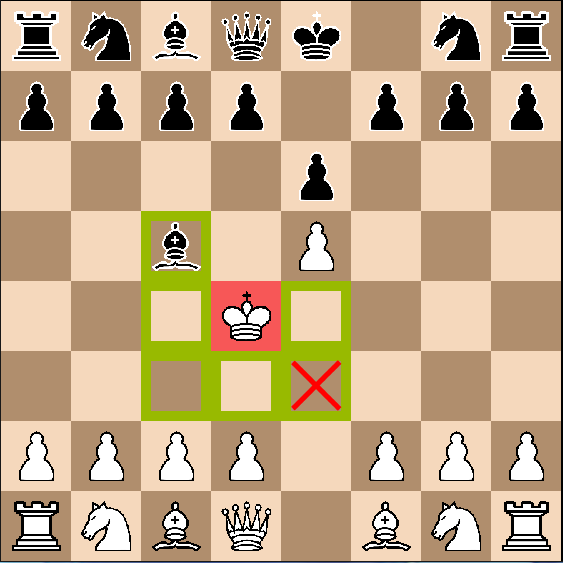
\includegraphics[scale=0.6]{assets/Bug_king_blocking.png}
\caption{Bug, König verhindert Schach}
\end{figure}

Um dieses Problem zu lösen hatte ich zunächst die Idee den König zu einer "transparenten
Figur" zu machen, sodass der Angriffszug auch durch diesen hindurch wirkt, doch ich sah immer
mehr Probleme kommen, die wieder aufwand gemacht hätten zu lösen, wie zum Beispiel, dass man die 
Figur, die vor dem König steht und das Schach verhindert nicht wegbewegt werden darf. Dann kam mir
aber die Idee, wie ich all diese Probleme auf einen Schlag lösen konnte.

\subsubsection{Foresight}
Wenn man es schaffen könnte, in die Zukunft nach dem nächsten Zug zu sehen und erkennen könnte, ob
der Zug als Konequenz hat, dass der König im Schach steht, könnte man diesen Zug verbieten. 
Genau das war der Gedanke hinter dieser Lösung. Ich lasse, bevor ich die möglichen Züge
einer Figur exportiere, die Liste durch einen Filter laufen, der oben Erwähntes prüft.
Der Filter sieht folgendermaßen aus:

\begin{lstlisting}
def filter_method_foresight(self, move):
        self.x, self.y = move #setting the position of the piece to the move, that you want to check
        ignoring_piece = None #currently no piece has to be ignored

        ### if you want to simulate to take a piece, 
        # without actually taking it, you can just 
        ### ignore it in the .detectingCheck method 
        for piece in Pieces.all_pieces_list:
        if (self.x, self.y) == (piece.x, piece.y) and not (piece == self):
                ignoring_piece = piece

        #checking if the king is checked, after the move
        Pieces.detectingCheck(ignoring_piece = ignoring_piece)

        white_check = bool(Pieces.white_is_checked)
        black_check = bool(Pieces.black_is_checked)
        white_bool = bool(self.farbe == (255,255,255))
        black_bool = bool(self.farbe == (0,0,0))

        #returning if the move is legal or not
        return (white_bool and not white_check) or (black_bool and not black_check)
\end{lstlisting}

Nachdem ich diesem Filter für jede Figur angewendet hatte, hatte ich keinerlei Probleme mehr mit
illegalen Zügen. 

\subsubsection{Stockfish}
Zunächst hatte ich noch an die Leinfachheit der Implementierung von Stockfish in
python geglaubt, aber ich sollte falsch liegen. Zunächst hatte ich Stockfish wie in
der Dokumentation beschrieben installiert und importiert. Als ich dann ein Objekt der
Klasse \glqq Stockfish\grqq{} erstellen wollte bekam ich folgende Fehlermeldung:
\begin{lstlisting}
        Traceback (most recent call last):
        File "D:\Julian\Coding\Sprachen\python\lib\site-packages\ stockfish\models.py", line 33, in __init__
        self.stockfish = subprocess.Popen(
        File "D:\Julian\Coding\Sprachen\python\lib\subprocess.py", line 947, in __init__
        self._execute_child(args, executable, preexec_fn, close_fds,
        File "D:\Julian\Coding\Sprachen\python\lib\subprocess.py", line 1416, in _execute_child
        hp, ht, pid, tid = _winapi.CreateProcess(executable, args,
        FileNotFoundError: [WinError 2] Das System kann die angegebene Datei nicht finden
        Exception ignored in: <function Stockfish.__del__ at 0x000001F7B592D820>
        Traceback (most recent call last):
        File "D:\Julian\Coding\Sprachen\python\lib\site-packages\ stockfish\models.py", line 270, in __del__
        self.stockfish.kill()
        AttributeError: 'Stockfish' object has no attribute 'stockfish'
\end{lstlisting}
Als ich nach Lösungen gesucht hatte, war ich in einem Forum auf User gestoßen,
die das selbe Problem hatten. Glücklicher Weise gab es die Möglichkeit eine .exe
Datei herunterzuladen und den Bot von dort aus zu starten. 

Ich fand die Lösung war nun nicht die Eleganteste, aber da das Programm für jeden
auszuführen sein soll, wollte ich nichts bei mir lokal bei dem Paket \glqq Stockfish\grqq{} ändern. 

\section{Danke an\dots{}}
Ich möchte zunächst dem Luisengymnasium und dem Kollegium, insbesondere Frau
Swiebodzinski, dafür danken, dass ich das Projekt in diesem Rahmen bearbeiten durfte. 
Ein besonderer Dank geht an zwei Mitschüler, Gero Beckmann und Vincent Piegsa, da ich
mich bei Fragen immer die Möglichkeit hatte mich an sie zu wenden.

Außerdem möchte ich den Usern der Medien Youtube, Reddit, Stackoverflow und GitHub bedanken,
da ich mir auch dort Hilfe holen konnte. 

\section{Schlusswort und Fazit}
Dieses Projekt war sehr anspruchsvoll, da ich das Schachprogramm \glqq from Scratch\grqq{}
gestartet habe und auf jegliche Hilfen von API's verzichtet habe. Dennoch war dieses Projekt
sehr Umfangreich und spannend, da ich das erste Mal im Frontend entwickelt habe und ich,
trotz vieler Hürden, meinen Spaß daran hatte. 

Ich bin mit dem Endresultat sehr zufrieden, obwohl mir es bis Dato  (\date) 
nicht gelungen ist, die Regel \glqq en passant \grqq{} zu implementieren.

\subsection{Zukünftige Aussichten}
Wie eben erwähnt habe ich vor die mir fehlende Regel einzubauen. Ebenfalls hatte ich vor
den Code nocheinmal aufzuräumen und zu kommentieren, um ihn für Interessierte nachvollziebarer
zu gestallten. 
Eine weitere Idee von mir war, dass ich eventuell das Programm auf meine eigene Website
hochlade und somit ein Onlinespiel zu schaffen.

%WAS HAB ICH GELERNT???


\end{document}